\begin{figure*}[hbtp]
  \centering
  \subfigure[Overall result]{
    \label{fig:8020-modularity--mean}
    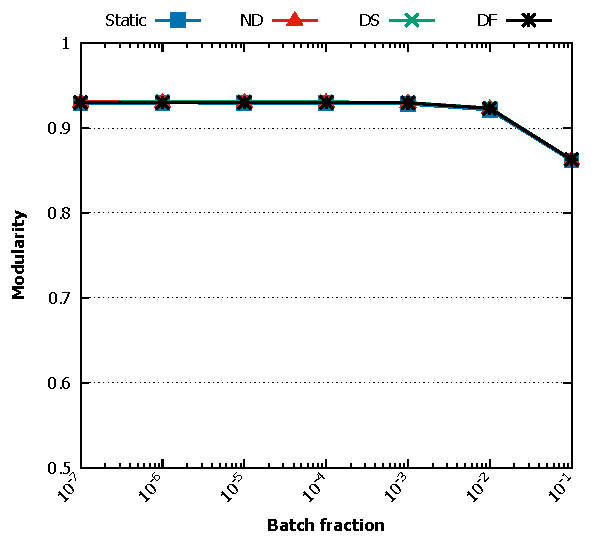
\includegraphics[width=0.38\linewidth]{out/8020-modularity-mean.pdf}
  }
  \subfigure[Results on each graph]{
    \label{fig:8020-modularity--all}
    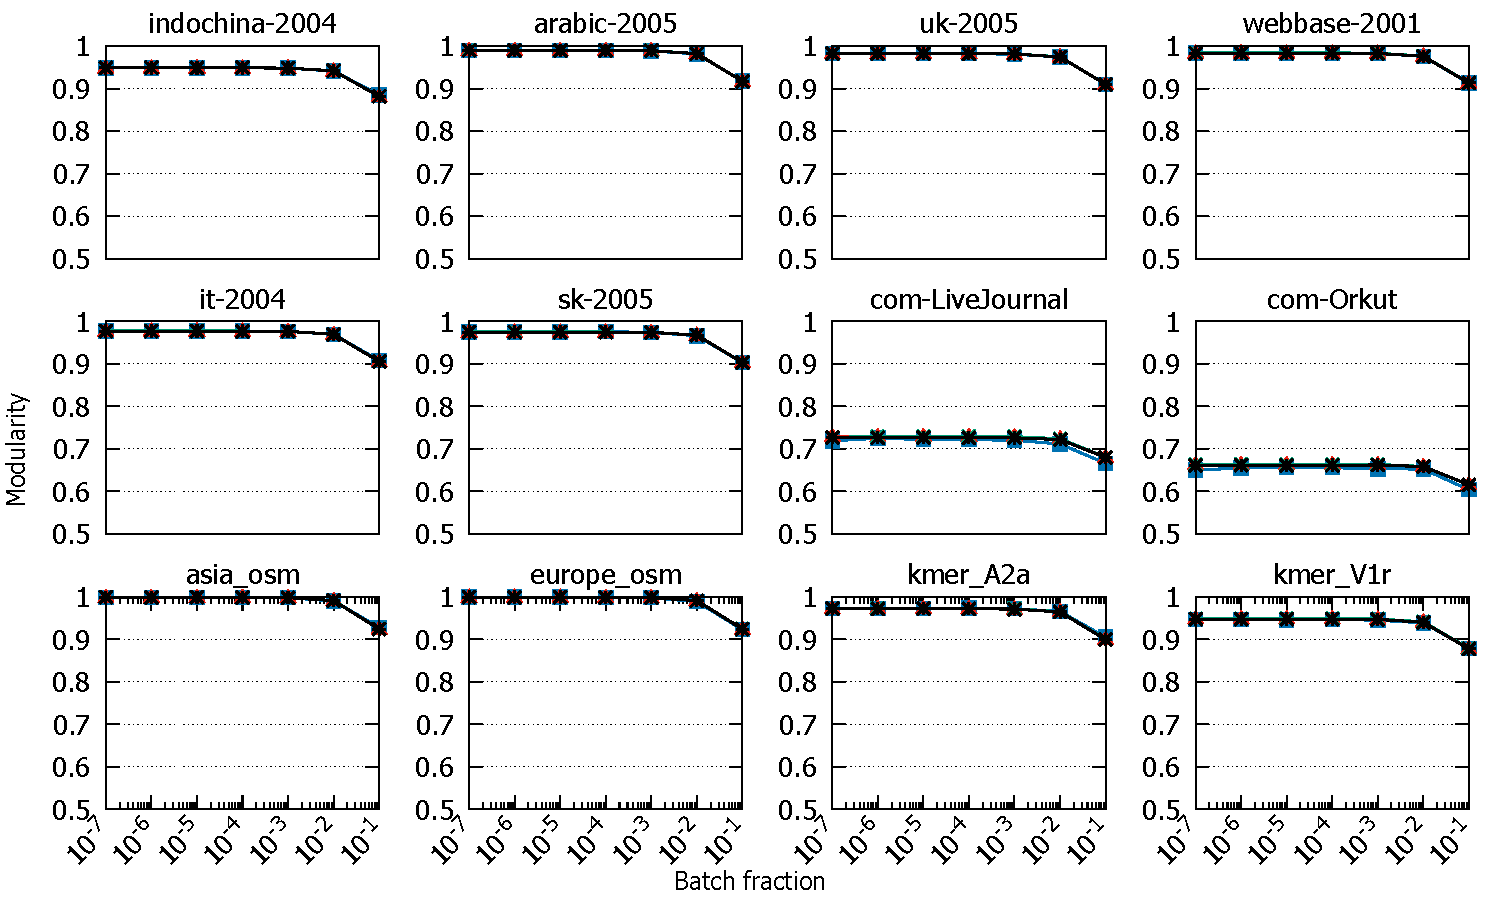
\includegraphics[width=0.58\linewidth]{out/8020-modularity-all.pdf}
  } \\[-2ex]
  \caption{Modularity comparison of our multicore implementation of \textit{Static}, \textit{Naive-dynamic (ND)}, \textit{Delta-screening (DS)}, and \textit{Dynamic Frontier (DF)} Louvain on large (static) graphs with generated random batch updates. The size of batch updates range from $10^{-7} |E|$ to $0.1 |E|$ in multiples of $10$ (logarithmic scale), consisting of $80\%$ edge insertions and $20\%$ edge deletions to simulate realistic dynamic graph updates. The right subfigure depicts the modularity for each approach in relation to each graph, while the left subfigure showcases overall modularity using arithmetic mean.}
  \label{fig:8020-modularity}
\end{figure*}
